\documentclass[10pt]{article}
\usepackage[utf8]{inputenc}
\usepackage[T1]{fontenc}
\usepackage{booktabs} % for better tables
\usepackage[]{minted}
\usepackage{amsmath}
\usepackage{amsfonts}
\usepackage{amssymb}
\usepackage[version=4]{mhchem}
\usepackage{stmaryrd}
\usepackage{bbold}
\usepackage{hyperref}
\hypersetup{colorlinks=true, linkcolor=blue, filecolor=magenta, urlcolor=cyan,}
\urlstyle{same}
\usepackage{graphicx}
\usepackage[export]{adjustbox}
\graphicspath{ {./images/} }
\newcommand{\norm}[1]{\left\lVert #1 \right\rVert}

\title{CM146, Winter 2024 \\
 Problem Set 4: Boosting, Unsupervised learning Due March 17, 11:59pm (Coding) }

\author{Harris Doan}
\date{March 15, 2024}


%New command to display footnote whose markers will always be hidden
\let\svthefootnote\thefootnote
\newcommand\blfootnotetext[1]{%
  \let\thefootnote\relax\footnote{#1}%
  \addtocounter{footnote}{-1}%
  \let\thefootnote\svthefootnote%
}

%Overriding the \footnotetext command to hide the marker if its value is `0`
\let\svfootnotetext\footnotetext
\renewcommand\footnotetext[2][?]{%
  \if\relax#1\relax%
    \ifnum\value{footnote}=0\blfootnotetext{#2}\else\svfootnotetext{#2}\fi%
  \else%
    \if?#1\ifnum\value{footnote}=0\blfootnotetext{#2}\else\svfootnotetext{#2}\fi%
    \else\svfootnotetext[#1]{#2}\fi%
  \fi
}

\begin{document}
\maketitle
\section*{Submission instructions}
\begin{itemize}
  \item Submit your solutions electronically on the course Gradescope site as PDF files.
  \item If you plan to typeset your solutions, please use the LaTeX solution template. If you must submit scanned handwritten solutions, please use a black pen on blank white paper and a high-quality scanner app.
  \item First three math heavy questions are due Friday March 15, 11:59pm. Coding/Implementation questions will be due on Sunday March 17, 11:59pm.
\end{itemize}

\section*{4 Implementation: Clustering and PCA [32 pts]}
Machine learning techniques have been applied to a variety of image interpretation problems. In this project, you will investigate facial recognition, which can be treated as a clustering problem ("separate these pictures of Joe and Mary").

For this project, we will use a small part of a huge database of faces of famous people (Labeled Faces in the Wild $[\mathrm{LFW}]$ people dataset ${ }^{1}$ ). The images have already been cropped out of the original image, and scaled and rotated so that the eyes and mouth are roughly in alignment; additionally, we will use a version that is scaled down to a manageable size of 50 by 37 pixels (for a total of 1850 "raw" features). Our dataset has a total of 1867 images of 19 different people. You will apply dimensionality reduction using principal component analysis (PCA) and explore clustering methods such as k-means and k-medoids to the problem of facial recognition on this dataset.

\section*{Starter Files}
code and data

\begin{itemize}
  \item Code: CS146-Winter2024-PS4.ipynb - Code for the Point, Cluster, and ClusterSet classes, on which you will build the clustering algorithms and the main code for the project.
  \item Utility code: \href{http://util.py}{util.py} - Utility methods for manipulating data, including through PCA.
\end{itemize}

Please use your @g.ucla.edu email id to access the code. Similar to previous problem sets, copy the colab notebook to your drive and make the changes. Mount the drive appropriately. To work on this HW: you need to download \href{http://util.py}{util.py} from here. Then, copy/upload this file to your own Google drive.

The notebook has marked blocks where you need to code.

$\# \# \#=========T O D O: S T A R T=========\# \# \#$

$\# \# \#=========T O D O: E N D==========\# \# \#$

Note: For the questions requiring you to complete a piece of code, you are expected to copy-paste your code as a part of the solution in the submission pdf. Tip: If you are using $\mathrm{IT}_{\mathbf{E}} \mathrm{X}$, check out the Minted package (example) for code highlighting.

Please note that you do not necessarily have to follow the skeleton code perfectly. We encourage you to include your own additional methods and functions. For this project, you are not allowed to use any scikit-learn classes or functions other than those already imported in the skeleton code.

\subsection*{4.1 PCA and Image Reconstruction [4 pts]}
Before attempting automated facial recognition, you will investigate a general problem with images. That is, images are typically represented as thousands (in this project) to millions (more generally) of pixel values, and a high-dimensional vector of pixels must be reduced to a reasonably lowdimensional vector of features.
\footnotetext{${ }^{1}$ \href{http://vis-www.cs.umass.edu/lfw/}{http://vis-www.cs.umass.edu/lfw/}
}
(a) As always, the first thing to do with any new dataset is to look at it. Use get\_lfw\_data (...) to get the LFW dataset with labels, and plot a couple of the input images using show\_image ( . . ). Then compute the mean of all the images, and plot it. (Remember to include all requested images in your writeup.) Comment briefly on this "average" face. \\

\section*{Solution 4.1a:}

\begin{figure}[H]
  \centering
  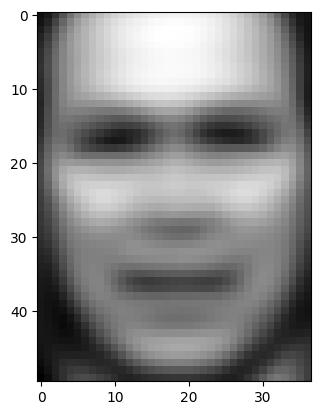
\includegraphics[width=5cm, height=5cm]{images/4.1a_mean_face.png}
  \caption{Mean Face}
  \label{fig:mean-face}
\end{figure}

The mean face definitely looks like a face from a distance, but very blurry. The dark spots being highlighted in the eyes and the mouth. It looks very uncanny valley and creepy almost. Stuff of nightmares. \\

Other faces included:

\begin{figure}[H]
  \centering
  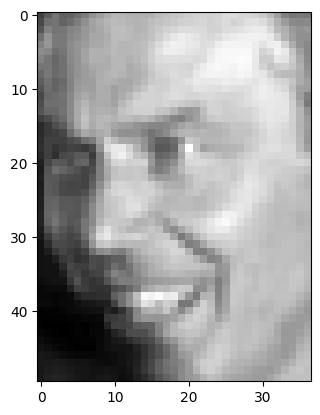
\includegraphics[width=5cm, height=5cm]{images/4.1a_face1.png}
  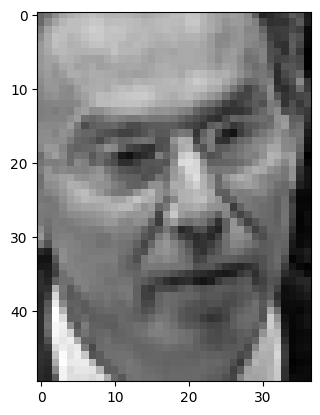
\includegraphics[width=5cm, height=5cm]{images/4.1a_face2.png}
  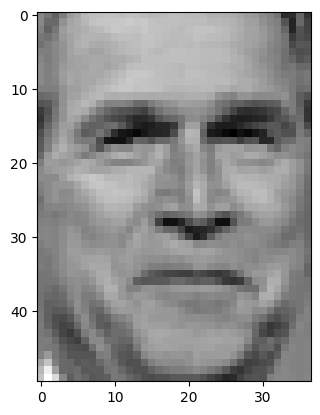
\includegraphics[width=5cm, height=5cm]{images/4.1a_face3.png}
  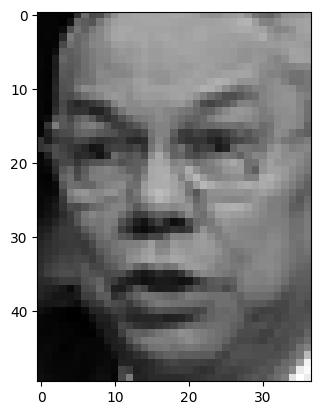
\includegraphics[width=5cm, height=5cm]{images/4.1a_face4.png}
  \caption{Other Sample Faces}
  \label{fig:sample-faces}
\end{figure}

\subsection*{4.1a Code}:
\begin{minted}[breaklines]{python}
    X, y = get_lfw_data()
    show_image(X[0])
    show_image(X[1])
    show_image(X[2])
    show_image(X[3])
    img_mean = np.mean(X, 0)
    show_image(img_mean)
\end{minted} 


(b) Perform PCA on the data using util.PCA(...). This function returns a matrix U whose columns are the principal components, and a vector mu which is the mean of the data. If you want to look at a principal component (referred to in this setting as an eigenface), run show\_image(vec\_to\_image(v)), where $\mathrm{v}$ is a column of the principal component matrix. (This function will scale vector $\mathrm{v}$ appropriately for image display.) Show the top twelve eigenfaces:

plot\_gallery([vec\_to\_image(U[:,i]) for i in range(12)])

Comment briefly on your observations. Why do you think these are selected as the top eigenfaces?

\section*{Solution 4.1b:}

\begin{figure}[H]
  \centering
  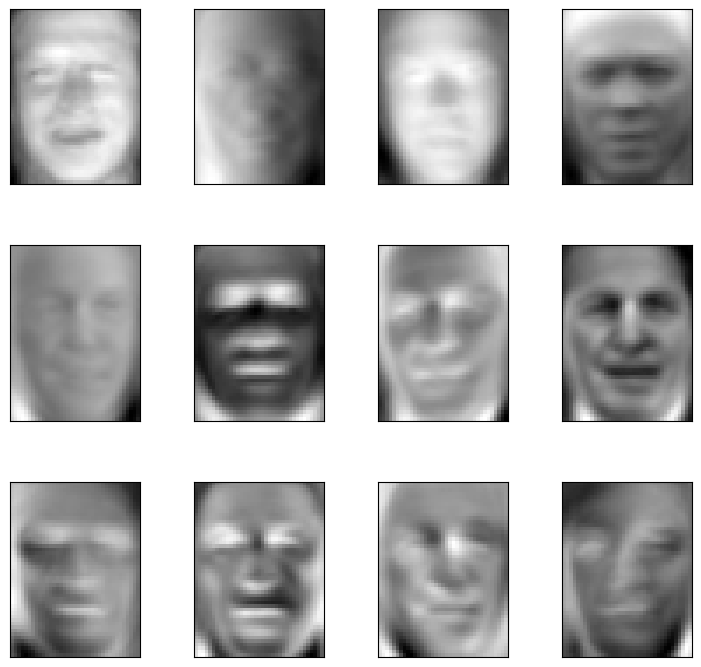
\includegraphics[width=5cm, height=5cm]{images/4.1b_eigen_faces.png}
  \caption{12 Eigenfaces}
  \label{fig:eigenfaces}
\end{figure}

Among the dozen images shown, each presents a unique variation: some are exceptionally illuminated or dimmed, and some portray the facial features with stark clarity or 
 lack of distinctiveness. The faces are also individually distinct. Likely, these images were selected for their pronounced uniqueness and variety, serving as archetypal eigenfaces. Given that Principal Component Analysis (PCA) was utilized, we can interpret that subsequent images will be characterized by attributes or components that are variations on these 12 foundational faces. \\

\subsection*{4.1b Code:}
\begin{minted}[breaklines]{python}
   U, mu = PCA(X)
   plot_gallery([vec_to_image(U[:,i]) for i in range(12)])
\end{minted} 

(c) Explore the effect of using more or fewer dimensions to represent images. Do this by:

\begin{itemize}
  \item Finding the principal components of the data
  \item Selecting a number $l$ of components to use
  \item Reconstructing the images using only the first $l$ principal components
  \item Visually comparing the images to the originals
\end{itemize}

To perform PCA, use apply\_PCA\_from\_Eig (... ) to project the original data into the lowerdimensional space, and then use reconstruct\_from\_PCA ( . . ) to reconstruct high-dimensional images out of lower dimensional ones. Then, using plotGallery ( . . ), submit a gallery of the first 12 images in the dataset, reconstructed with $l$ components, for $l=1,10,50,100,500,1288$. Comment briefly on the effectiveness of differing values of $l$ with respect to facial recognition.

We will revisit PCA in the last section of this project.

\section*{Solution 4.1c:}

The images reveal that clarity and detail improve as the "l" value rises, indicating a preservation of more original image data. "L" represents the number of retained image components, which explains why at "l" equals 1, the images resemble each other and the mean face, preserving only the most crucial component. In contrast, at "l" values of 500 and 1288, the images become sharper and more individualized. However, the minimal difference observed between "l" at 500 and 1288 implies diminishing benefits beyond "l" equals 500. For facial recognition, too low an "l" value homogenizes the images, while too high an "l" value, such as 1288, offers little extra detail and could hinder performance by including unnecessary components. \\

\begin{figure}[H]
  \centering
  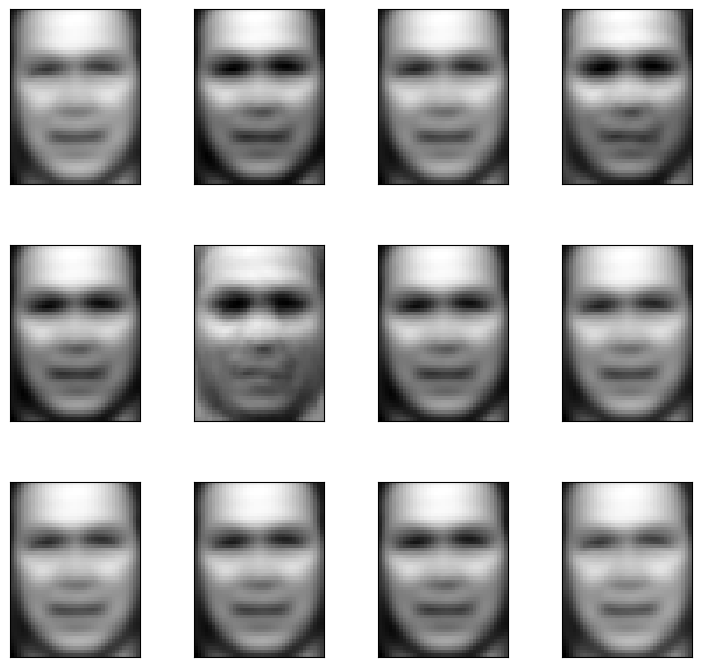
\includegraphics[width=5cm, height=5cm]{images/4.1c_1.png}
  \caption{l = 1}
  \label{fig:faces}
\end{figure}

\begin{figure}[H]
  \centering
  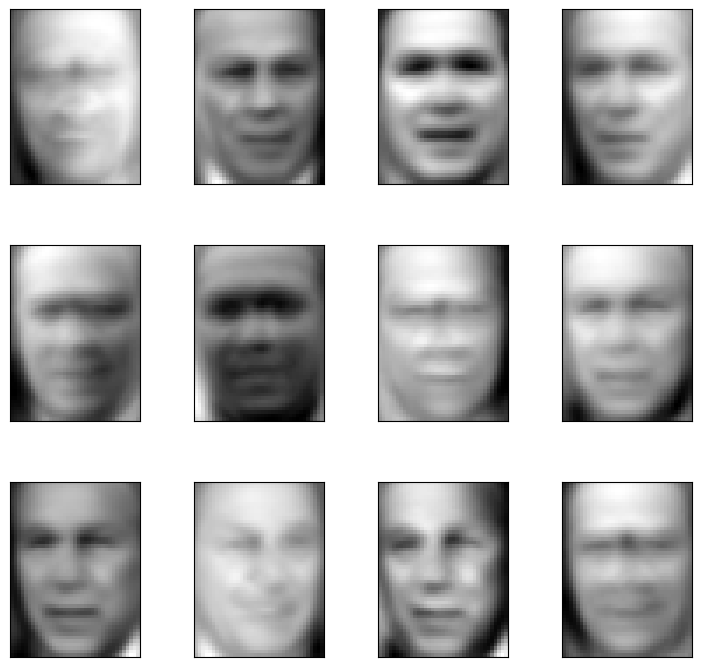
\includegraphics[width=5cm, height=5cm]{images/4.1c_2.png}
  \caption{l = 10}
  \label{fig:faces}
\end{figure}

\begin{figure}[H]
  \centering
  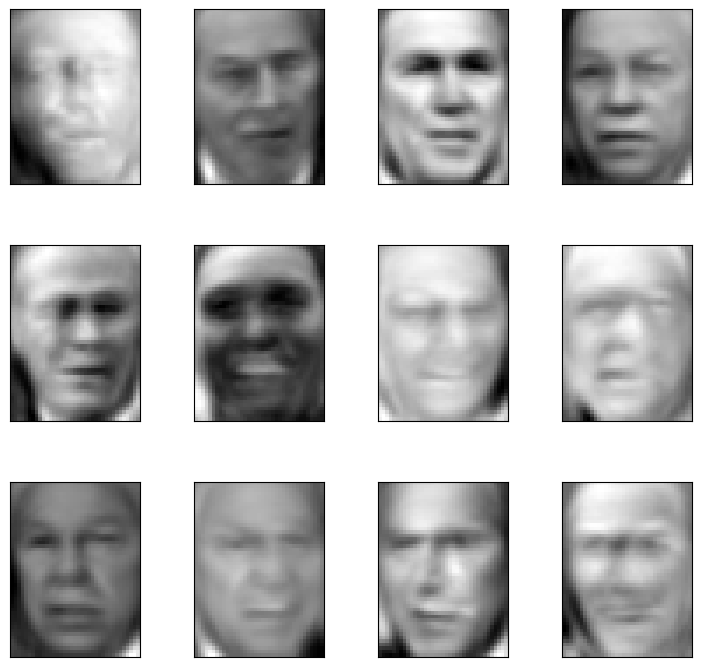
\includegraphics[width=5cm, height=5cm]{images/4.1c_3.png}
  \caption{l = 50}
  \label{fig:faces}
\end{figure}

\begin{figure}[H]
  \centering
  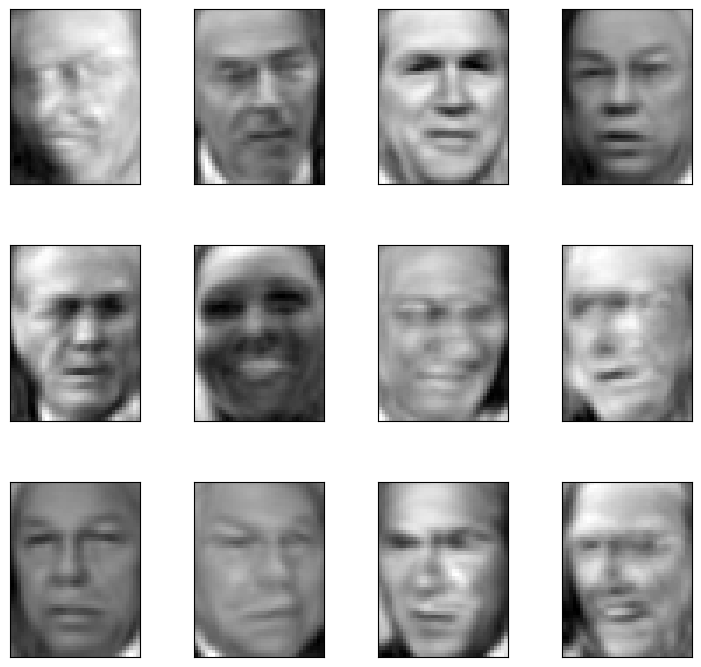
\includegraphics[width=5cm, height=5cm]{images/4.1c_4.png}
  \caption{l = 100}
  \label{fig:faces}
\end{figure}

\begin{figure}[H]
  \centering
  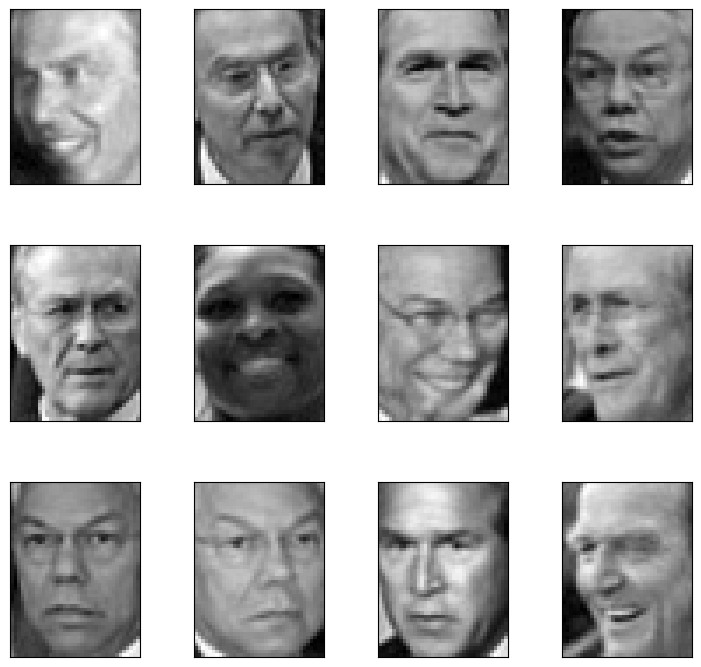
\includegraphics[width=5cm, height=5cm]{images/4.1c_5.png}
  \caption{l = 100}
  \label{fig:faces}
\end{figure}

\begin{figure}[H]
  \centering
  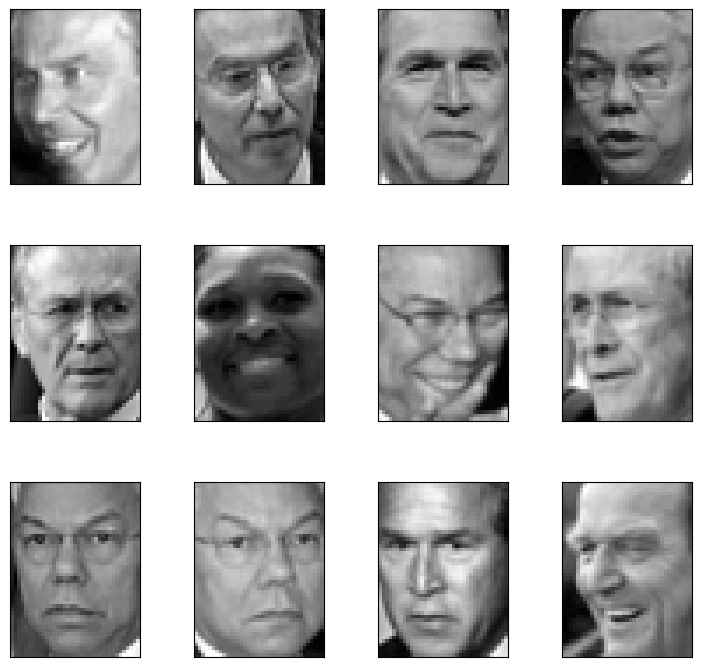
\includegraphics[width=5cm, height=5cm]{images/4.1c_6.png}
  \caption{l = 1288}
  \label{fig:faces}
\end{figure}

\subsection*{4.1c Code:}
\begin{minted}[breaklines]{python}
l_values = [1, 10, 50, 100, 500, 1288]
     for l_value in l_values:
         Z, UI = apply_PCA_from_Eig(X, U, l_value, mu)
         X_rec = reconstruct_from_PCA(Z, UI, mu)
         title = f"l = {l_value}"
         plot_gallery(X_rec, title=title)
\end{minted} 

\section*{4.2 $K$-Means and $K$-Medoids $[16 \mathrm{pts}]$}
Next, we will explore clustering algorithms in detail by applying them to a toy dataset. In particular, we will investigate $k$-means and $k$-medoids (a slight variation on $k$-means).


(a) In $k$-means, we attempt to find $k$ cluster centers $\boldsymbol{\mu}_{j} \in \mathbb{R}^{d}, j \in\{1, \ldots, k\}$ and $n$ cluster assignments $c^{(i)} \in\{1, \ldots, k\}, i \in\{1, \ldots, n\}$, such that the total distance between each data point and the nearest cluster center is minimized. In other words, we attempt to find $\boldsymbol{\mu}_{1}, \ldots, \boldsymbol{\mu}_{k}$ and $c^{(1)}, \ldots, c^{(n)}$ that minimizes

$$
J(\boldsymbol{c}, \boldsymbol{\mu})=\sum_{i=1}^{n}\left\|\boldsymbol{x}^{(i)}-\boldsymbol{\mu}_{c^{(i)}}\right\|^{2}
$$

To do so, we iterate between assigning $\boldsymbol{x}^{(i)}$ to the nearest cluster center $c^{(i)}$ and updating each cluster center $\boldsymbol{\mu}_{j}$ to the average of all points assigned to the $j^{\text {th }}$ cluster.

Instead of holding the number of clusters $k$ fixed, one can think of minimizing the objective function over $\boldsymbol{\mu}, \boldsymbol{c}$, and $k$. Show that this is a bad idea. Specifically, what is the minimum possible value of $J(\boldsymbol{c}, \boldsymbol{\mu}, k)$ ? What values of $\boldsymbol{c}, \boldsymbol{\mu}$, and $k$ result in this value?\\

\section*{Solution 4.2a:}

The minimum value achievable by the objective function $J(c, \mu, k)$, when adjusting $k$, is $0$. This scenario occurs when $k$ is set equal to the number of data points, $n$, effectively assigning each point to its unique cluster. In this case, since every cluster contains exactly one data point, the distance between any point in a cluster and its centroid is zero, resulting in $J(c, \mu, k) = 0$. This situation is analogous to overfitting in a model, such as fitting an $n$-degree polynomial to a dataset comprising $n$ points. The conditions for achieving $J(c, \mu, k) = 0$ are specified as follows: $c(i) = i$, $\mu_i = x_i$, and $k = n$, where $x_i$ denotes a data point in the dataset. \\

(b) To implement our clustering algorithms, we will use Python classes to help us define three abstract data types: Point, Cluster, and ClusterSet. Read through the documentation for these classes. (You will be using these classes later, so make sure you know what functionality each class provides!) Some of the class methods are already implemented, and other methods are described in comments. Implement all of the methods marked TODO in the Cluster and ClusterSet classes.

\section*{Solution 4.2b:}

\subsection*{Cluster: def centroid(self):}

\begin{minted}[breaklines]{python}
    def centroid(self) :
        """
        Compute centroid of this cluster.

        Returns
        --------------------
            centroid -- Point, centroid of cluster
        """

        ### ========== TODO : START ========== ###
        # part 2b: implement
        # set the centroid label to any value (e.g. the most common label in this cluster)
        #attrs = [np.mean([p.attrs[i] for p in self.points]) for i in range(len(self.points[0].attrs))]
        all_attrs = np.array([p.attrs for p in self.points])
        attrs = np.mean(all_attrs, axis = 0)

        label = stats.mode([p.label for p in self.points])
        name = label
        centroid = Point(name, label, attrs)
        return centroid
        ### ========== TODO : END ========== ###
\end{minted} 

\subsection*{Cluster: def medoid(self):}

\begin{minted}[breaklines]{python}
    def medoid(self) :
        """
        Compute medoid of this cluster, that is, the point in this cluster
        that is closest to all other points in this cluster.

        Returns
        --------------------
            medoid -- Point, medoid of this cluster
        """

        ### ========== TODO : START ========== ###
        # part 2b: implement
        pairwise_dist_matrix = []
        for p in self.points:
          temp_lst = []
          for p2 in self.points:
            temp_lst.append(p.distance(p2))
          pairwise_dist_matrix.append(temp_lst)
        row_sums = np.sum(pairwise_dist_matrix, axis=0).tolist()
        medoid = self.points[np.nanargmin(row_sums)]
        return medoid
        ### ========== TODO : END ========== ###
\end{minted}

\subsection*{ClusterSet: def centroid(self):}

\begin{minted}[breaklines]{python}
    def centroids(self) :
        """
        Return centroids of each cluster in this cluster set.

        Returns
        --------------------
            centroids -- list of Points, centroids of each cluster in this cluster set
        """

        ### ========== TODO : START ========== ###
        # part 2b: implement
        centroids = [m.centroid() for m in self.members]
        return centroids
        ### ========== TODO : END ========== ###
\end{minted}


\subsection*{ClusterSet: def medoid(self):}

\begin{minted}[breaklines]{python}
    def medoids(self) :
        """
        Return medoids of each cluster in this cluster set.

        Returns
        --------------------
            medoids -- list of Points, medoids of each cluster in this cluster set
        """

        ### ========== TODO : START ========== ###
        # part 2b: implement
        medoids = [m.medoid() for m in self.members]
        return medoids
        ### ========== TODO : END ========== ###
\end{minted}

(c) Next, implement random\_init(...) and kMeans (...) based on the specifications provided in the code.

\section*{Solution 4.2c:}

\subsection*{def random\textunderscore init(points, k):}
\begin{minted}[breaklines]{python}
def random_init(points, k) :
    """
    Randomly select k unique elements from points to be initial cluster centers.

    Parameters
    --------------------
        points         -- list of Points, dataset
        k              -- int, number of clusters

    Returns
    --------------------
        initial_points -- list of k Points, initial cluster centers
    """
    ### ========== TODO : START ========== ###
    # part 2c: implement (hint: use np.random.choice)
    return np.random.choice(points, size=k, replace=False).tolist()
    ### ========== TODO : END ========== ###
\end{minted}

\subsection*{def kMeans(points, k, init='random', plot=False):}
\begin{minted}[breaklines]{python}
def kMeans(points, k, init='random', plot=False) :
    """
    Cluster points into k clusters using variations of k-means algorithm.

    Parameters
    --------------------
        points  -- list of Points, dataset
        k       -- int, number of clusters
        average -- method of ClusterSet
                   determines how to calculate average of points in cluster
                   allowable: ClusterSet.centroids, ClusterSet.medoids
        init    -- string, method of initialization
                   allowable:
                       'cheat'  -- use cheat_init to initialize clusters
                       'random' -- use random_init to initialize clusters
        plot    -- bool, True to plot clusters with corresponding averages
                         for each iteration of algorithm

    Returns
    --------------------
        k_clusters -- ClusterSet, k clusters
    """

    ### ========== TODO : START ========== ###
    # part 2c: implement
    # Hints:
    #   (1) On each iteration, keep track of the new cluster assignments
    #       in a separate data structure. Then use these assignments to create
    #       a new ClusterSet object and update the centroids.
    #   (2) Repeat until the clustering no longer changes.
    #   (3) To plot, use plot_clusters(...).
    #average = ClusterSet.centroids #or ClusterSet.medoids
    return kAverages(points, k, ClusterSet.centroids, init, plot)
\end{minted}

(d) Now test the performance of $k$-means on a toy dataset.

Use generate\_points\_2d(...) to generate three clusters each containing 20 points. (You can modify generate\_points\_2d(...) to test different inputs while debugging your code, but be sure to return to the initial implementation before creating any plots for submission.) You can plot the clusters for each iteration using the plot\_clusters (...) function.

In your writeup, include plots for the $k$-means cluster assignments and corresponding cluster "centers" for each iteration when using random initialization and " $\mathrm{k}=3$ ".

\section*{Solution 4.2d:}

The set of clusters stabilized after three iterations; the values in the fourth iteration were identical to those in the third. Therefore, the cluster plot produced from the third iteration would look identical to the fourth iteration. \\

\begin{figure}[H]
  \centering
  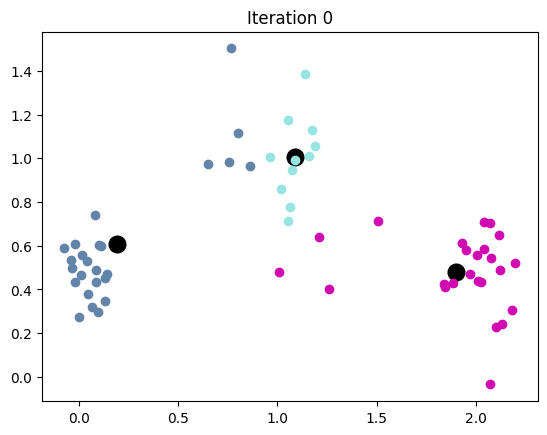
\includegraphics[width=7cm, height=7cm]{images/4.2d_1.png}
  \caption{Iteration 1}
  \label{fig:Clusters}
\end{figure}

\begin{figure}[H]
  \centering
  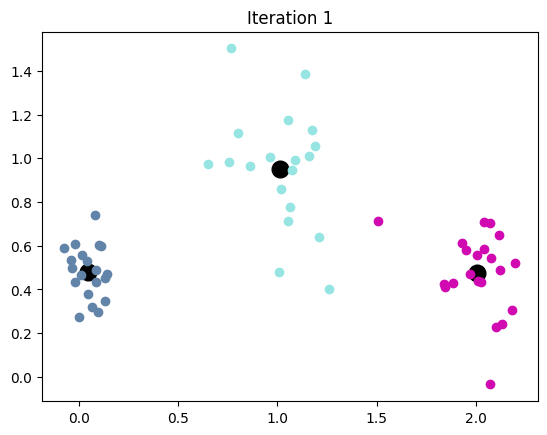
\includegraphics[width=7cm, height=7cm]{images/4.2d_2.png}
  \caption{Iteration 2}
  \label{fig:Clusters}
\end{figure}

\begin{figure}[H]
  \centering
  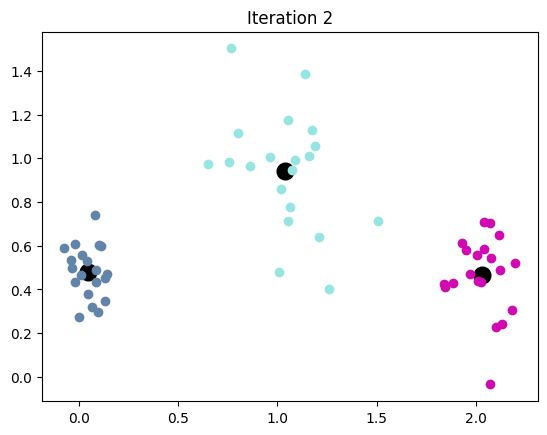
\includegraphics[width=7cm, height=7cm]{images/4.2d_3.png}
  \caption{Iteration 3}
  \label{fig:Clusters}
\end{figure}

(e) Implement kMedoids (...) based on the provided specification.

$H i n t$ : Since $k$-means and $k$-medoids are so similar, you may find it useful to refactor your code to use a helper function kAverages (points, k, average, init='random', plot=False), where average is a method that determines how to calculate the average of points in a cluster (so it can take on values ClusterSet.centroids or ClusterSet.medoids). ${ }^{2}$

As before, include plots for $k$-medoids clustering for each iteration when using random initialization and " $\mathrm{k}=3$ ".

\section*{Solution 4.2e:}

\subsection*{def kMedoids(points, k, init='random', plot=False):}
\begin{minted}[breaklines]{python}
def kMedoids(points, k, init='random', plot=False) :
    """
    Cluster points in k clusters using k-medoids clustering.
    See kMeans(...).
    """
    ### ========== TODO : START ========== ###
    # part 2e: implement

    #k_clusters = ClusterSet()
    #return k_clusters
    return kAverages(points, k, ClusterSet.medoids, init, plot)

    ### ========== TODO : END ========== ###
\end{minted}

\subsection*{def kAverages(points, k, average, init='random', plot=False):}
\begin{minted}[breaklines]{python}
def kMeans(points, num_clusters, find_averages, start='random', show_plot=True):
    point_groups = {}
    if start == 'cheat':
        chosen_starts = cheat_start(points)
    elif start == 'random':
        chosen_starts = random_start(points, num_clusters)

    for start_pt in chosen_starts:
        point_groups[start_pt] = []

    for point in points:
        distance_list = [point.distance(centroid) for centroid in chosen_starts]
        nearest_centroid = chosen_starts[np.nanargmin(distance_list)]
        point_groups[nearest_centroid].append(point)

    cluster_group = ClusterSet()
    for group in point_groups.values():
        cluster_group.add(Cluster(group))

    iteration_count = 0
    while True:

        if show_plot:
            plot_clusters(cluster_group, "Iteration " + str(iteration_count), find_averages)
        iteration_count += 1

        new_assignments = {}
        new_chosen_starts = find_averages(cluster_group)
        for start_pt in new_chosen_starts:
            new_assignments[start_pt] = []

        for point in points:
            distance_list = [point.distance(centroid) for centroid in new_chosen_starts]
            closest_centroid = new_chosen_starts[np.nanargmin(distance_list)]
            new_assignments[closest_centroid].append(point)

        new_cluster_group = ClusterSet()
        for group in new_assignments.values():
            new_cluster_group.add(Cluster(group))

        if new_cluster_group.same_as(cluster_group):
            break
        else:
            cluster_group = new_cluster_group

    if find_averages == ClusterSet.centroids:
        print("kMeans: " + str(iteration_count))
    else:
        print("kMedoids: " + str(iteration_count))
    final_clusters = cluster_group

    return final_clusters
\end{minted}

\begin{figure}[H]
  \centering
  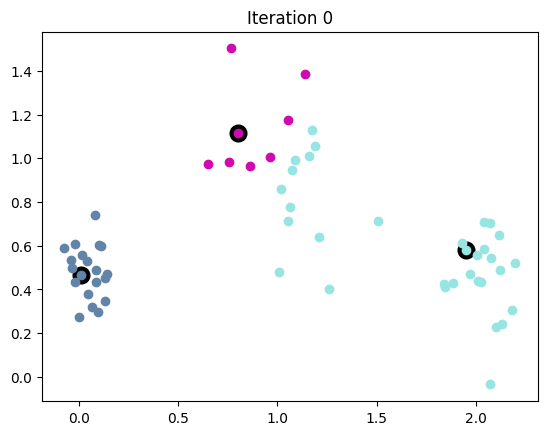
\includegraphics[width=7cm, height=7cm]{images/4.2e_1.png}
  \caption{Iteration 1}
  \label{fig:Clusters}
\end{figure}

\begin{figure}[H]
  \centering
  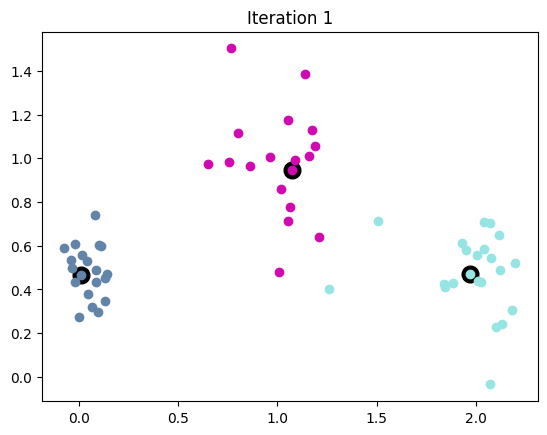
\includegraphics[width=7cm, height=7cm]{images/4.2e_2.png}
  \caption{Iteration 2}
  \label{fig:Clusters}
\end{figure}

\begin{figure}[H]
  \centering
  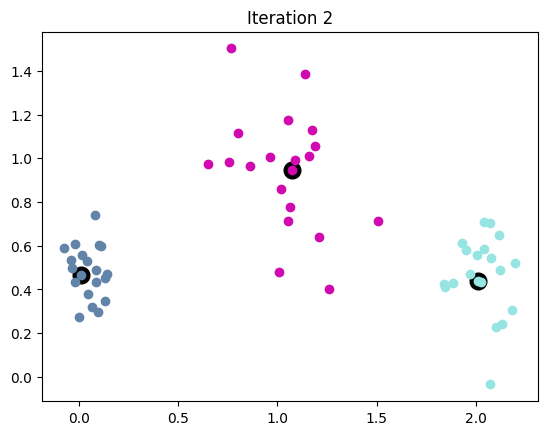
\includegraphics[width=7cm, height=7cm]{images/4.2e_3.png}
  \caption{Iteration 3}
  \label{fig:Clusters}
\end{figure}

Analogous to part (d), stability in the cluster set was achieved after three iterations, with the fourth iteration yielding values that were identical to those of the third. \\

(f) Finally, we will explore the effect of initialization. Implement cheat\_init (...).

Now compare clustering by initializing using cheat\_init(...). Include plots for $k$-means and $k$-medoids using " $\mathrm{k}=3$ " for each iteration.

\section*{Solution 4.2f:}

\subsection*{def cheat\textunderscore init(points):}
\begin{minted}[breaklines]{python}
def cheat_init(points) :
    """
    Initialize clusters by cheating!

    Details
    - Let k be number of unique labels in dataset.
    - Group points into k clusters based on label (i.e. class) information.
    - Return medoid of each cluster as initial centers.

    Parameters
    --------------------
        points         -- list of Points, dataset

    Returns
    --------------------
        initial_points -- list of k Points, initial cluster centers
    """
    ### ========== TODO : START ========== ###
    # part 2f: implement
    initial_points = []
    labels = list(set([p.label for p in points]))
    for l in labels:
      c = Cluster([p for p in points if p.label == l])
      initial_points.append(c.medoid())

    return initial_points
    ### ========== TODO : END ========== ###
\end{minted}

\begin{figure}[H]
  \centering
  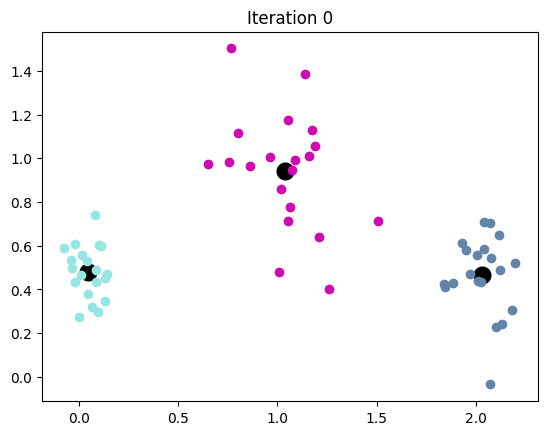
\includegraphics[width=7cm, height=7cm]{images/4.2f_Means.png}
  \caption{kMeans}
  \label{fig:Clusters}
\end{figure}

\begin{figure}[H]
  \centering
  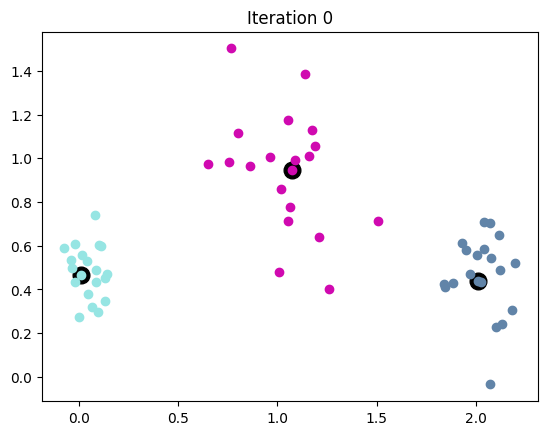
\includegraphics[width=7cm, height=7cm]{images/4.2f_Medoids.png}
  \caption{kMedoids}
  \label{fig:Clusters}
\end{figure}

The K-means process concluded in just two iterations, hinting that the cluster formation achieved in the initial pass was definitive. The purpose of the subsequent iteration was to ensure the stability of the initial findings. Similarly, with centers set through a predetermined method for K-medoids, convergence was achieved in a single iteration, but a second iteration was carried out to verify the consistency of the outcomes between the first and second iterations. \\


\subsection*{4.3 Clustering Faces [12 pts]}
Finally (!), we will apply clustering algorithms to the image data. To keep things simple, we will only consider data from four individuals. Make a new image dataset by selecting 40 images each from classes $4,6,13$, and 16 , then translate these images to (labeled) points: ${ }^{3}$

$\mathrm{X} 1, \mathrm{y} 1$ = util.limit\_pics(X, y, [4, 6, 13, 16], 40)

points = build\_face\_image\_points(X1, y1)

(a) Apply $k$-means and $k$-medoids to this new dataset with $k=4$ and initializing the centroids randomly. Evaluate the performance of each clustering algorithm by computing the average
\footnotetext{${ }^{2}$ In Python, if you have a function stored to the variable func, you can apply it to parameters arg by calling func(arg). This works even if func is a class method and arg is an object that is an instance of the class.

${ }^{3}$ There is a bug in fetch\_lfw version 0.18 .1 where the results of the loaded images are not always in the same order. This is not a problem for the previous parts but can affect the subset selected in this part. Thus, you may see varying results. Results that show the correct qualitative behavior will get full credit.
}
cluster purity with ClusterSet.score (...). As the performance of the algorithms can vary widely depending upon the initialization, run both clustering methods 10 times and report the average, minimum, and maximum performance along with runtime. How do the clustering methods compare in terms of clustering performance and runtime?

\begin{center}
\begin{tabular}{l|lllll}
 & average purity & $\min$ purity & $\max$ purity & average time & $\min$ time $\max$ time \\
\hline
$k$-means &  &  &  &  &  \\
\hline
\end{tabular}
\end{center}

Now construct another dataset by selecting 40 images each from two individuals 4 and 13 .

\section*{Solution 4.3a:}

\begin{center}
\begin{tabular}{l|llllll}
 & average purity & $\min$ purity & $\max$ purity & average time & $\min$ time & $\max$ time \\
\hline
$k$-means & 0.583 & 0.51875  & 0.6875  & 21.9425  & 13.3779 & 35.9079 \\
$k$-medoids & 0.638  & 0.54375 & 0.75625 & 25.7866  & 18.2844 & 40.8492  \\
\hline
\end{tabular}
\end{center}

Based on the information in the table, k-means and k-medoids show comparable levels of performance. Nonetheless, k-means edges out slightly as the superior choice, evidenced by its marginally better average clustering performance score, reduced runtime, and superior maximum score. Despite k-means having a slightly longer maximum runtime compared to k-medoids, the average performance score and runtime serve as the most dependable metrics for assessing efficiency and speed in this context. \\

(b) Explore the effect of lower-dimensional representations on clustering performance. To do this, compute the principal components for the entire image dataset, then project the newly generated dataset into a lower dimension (varying the number of principal components), and compute the scores of each clustering algorithm.

So that we are only changing one thing at a time, use init= ' cheat' to generate the same initial set of clusters for $k$-means and $k$-medoids. For each value of $l$, the number of principal components, you will have to generate a new list of points using build\_face\_image\_points (...).) Let $l=1,3,5, \ldots, 49$. The number of clusters $K=2$. Then, on a single plot, plot the clustering score versus the number of components for each clustering algorithm (be sure to label the algorithms). Discuss the results in a few sentences.

Some pairs of people are more similar to one another and some more different.

\section*{Solution 4.3b:}

\begin{figure}[H]
  \centering
  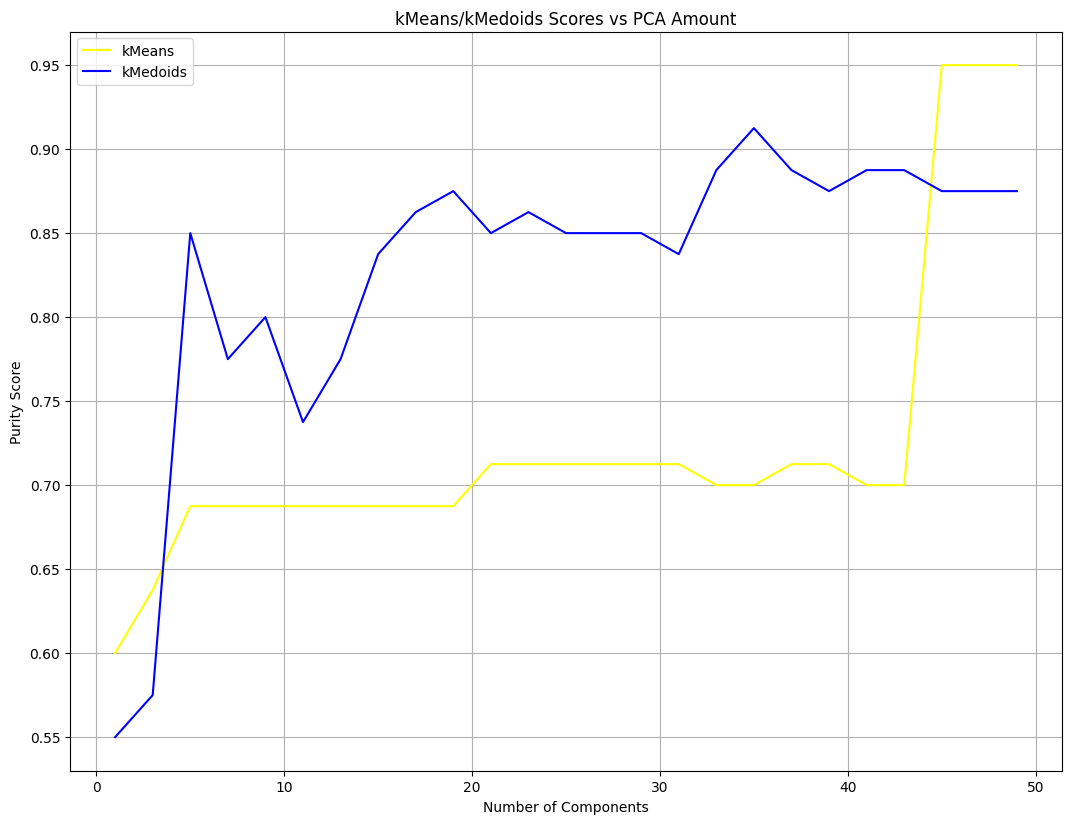
\includegraphics[width=10cm, height=10cm]{images/4.3b_graph.png}
  \caption{Number of Components vs Purity Score}
  \label{fig:Clusters}
\end{figure}

With the increment in the number of principal components, there is a noticeable improvement in the performance of both K-means and K-medoids. This improvement makes sense as retaining more data allows these methods to more effectively discern the similarities and differences among the image data points. Furthermore, K-medoids typically surpasses K-means in performance, with two exceptions: 1) when employing only the first principal component, and 2) when a substantial number of principal components (45 or more) are used. Initially, the performance disparity between the two methods is slight (up to approximately \(l \leq 5\)). However, as \(l\) grows from 5 to 40, the performance differential significantly expands, then narrows again past the 40-component mark, at which point K-means starts to outshine. It's plausible that K-medoids often leads because, in facial recognition scenarios, having the cluster center as an actual data point rather than a computed average may offer an advantage. \\


(c) Experiment with the data to find a pair of individuals that clustering can discriminate very well and another pair that it finds very difficult (assume you have 40 images for each individual, projected to the top 50 principal components space). Describe your methodology (you may choose any of the clustering algorithms you implemented). Report these twp pairs of individuals (most similar pair and most discriminative pair) in your writeup (display each pair of images using plot\_representative\_images), and comment briefly on the results.

\section*{Solution 4.3c:}

I proceeded by pairing each possible combination of individuals from the dataset, taking 40 images per individual as done previously, and merging them into a single dataset for analysis. I then applied the K-medoids algorithm, configured for two clusters to reflect the pair being analyzed, and utilized a 'cheating' initialization to maintain consistency in starting conditions across tests. Based on earlier observations that K-medoids tends to outperform K-means, I opted for this method for its reliability. After executing the algorithm for each pair, I recorded their clustering scores, identifying which pair yielded the highest and lowest scores respectively. The pair that stood out the most was between individuals 0 and 6 (achieving a score of 0.9875), where the distinction was immediately evident due to their contrasting orientations and gender, leading to distinct facial features that facilitated their separation into distinct clusters. On the opposite end, the pair of individuals 1 and 8 (scoring 0.5125) presented a challenge due to their similarities—both being males with comparable facial expressions and features, making it challenging for K-medoids to distinctly categorize their features into separate clusters, hence the lower score. \\

\begin{figure}[H]
  \centering
  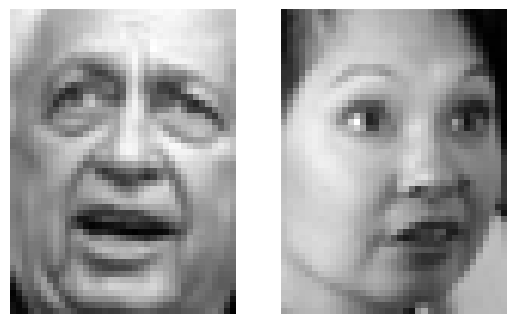
\includegraphics[width=10cm, height=10cm]{images/4.3c_1_3.png}
  \caption{Easy to Differentiate}
  \label{fig:Clusters}
\end{figure}

\begin{figure}[H]
  \centering
  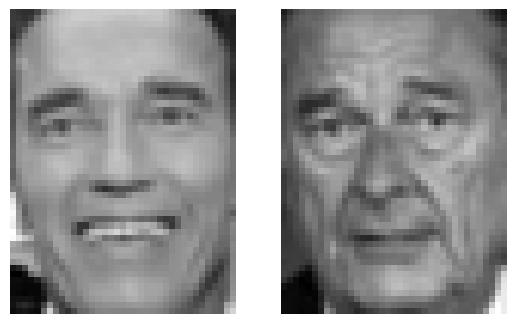
\includegraphics[width=10cm, height=10cm]{images/4.3c_2_6.png}
  \caption{Difficult to Differentiate}
  \label{fig:Clusters}
\end{figure}

\end{document}